\documentclass{standalone}

\usepackage[dvipsnames]{xcolor}
\usepackage{pgfplots}
\usepackage{tikz}

\begin{document}

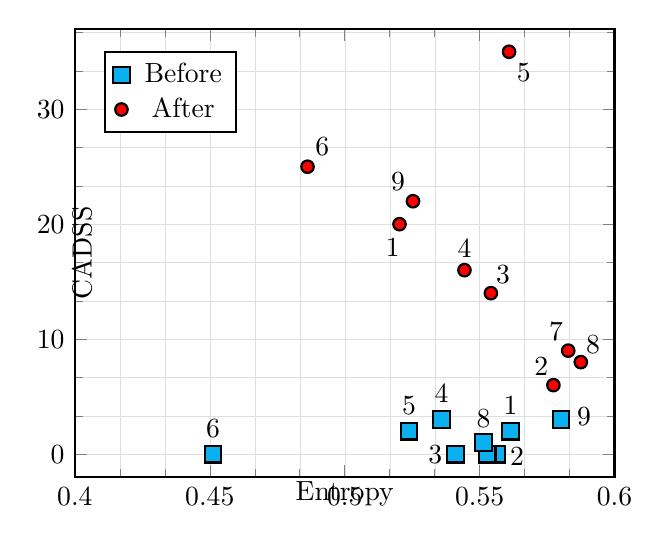
\begin{tikzpicture}
\begin{axis}
	[
	legend style = { at = {(0.30, 0.95) }},
	minor tick num=2,
	thick,
	xlabel = Entropy,
	ylabel = CADSS,
	xmax = 0.6, xmin = 0.4,
	ymax = 37, ymin = -2,
	x label style={at={(axis description cs:0.5,0.0125)}},
	y label style={at={(axis description cs:0.05,0.5)}},
	grid=both,
    grid style={line width=.1pt, draw=gray!25},
	]
    
% Before:
	\node at (axis cs: 0.56149, 2.0+2.25){1};
	\node at (axis cs: 0.55639+0.0075, 0.0-0.25){2};
	\node at (axis cs: 0.54105-0.0075, 0.0){3};
	\node at (axis cs: 0.53585, 3.0+2.25){4};
	\node at (axis cs: 0.5238, 2.0+2.25){5};
	\node at (axis cs: 0.45117, 0.0+2.25){6};
%	\node at (axis cs: 0.55283, 0.0+2.25){7}; % Subject 7 is better left out
	\node at (axis cs: 0.55144, 1.0+2.125){8};
	\node at (axis cs: 0.58017+0.0085, 3.0+0.25){9}; 	

% After:
	\node at (axis cs: 0.5203-0.0025, 20.0-2.00){1};
	\node at (axis cs: 0.57734-0.0045, 6.0+1.65){2};
	\node at (axis cs: 0.55417+0.0045, 14.0+1.65){3};
	\node at (axis cs: 0.54437, 16.0+1.85){4};
	\node at (axis cs: 0.56091+0.0055, 35.0-1.85){5};
	\node at (axis cs: 0.48621+0.0055, 25.0+1.75){6};
	\node at (axis cs: 0.58283-0.0045, 9.0+1.65){7};
	\node at (axis cs: 0.5875+0.0045, 8.0+1.55){8};
	\node at (axis cs: 0.5253-0.0055, 22.0+1.75){9};
 
    	
	\addplot[
	color = black,
	fill = ProcessBlue,
	mark = square*, % A filled square
	mark size = 3pt,
	only marks
	] coordinates {
	( 0.56149, 2.0 )
	( 0.55639, 0.0 )
	( 0.54105, 0.0 )
	( 0.53585, 3.0 )
	( 0.52380, 2.0 )
	( 0.45117, 0.0 )
	( 0.55283, 0.0 )
	( 0.55144, 1.0 )
	( 0.58017, 3.0 )
	};
	
	\addplot[
	color = black,
	fill = red,
	mark = *, % A filled circle
	mark size = 2.25pt,
	only marks
	] coordinates {
	( 0.52030, 20.0 )
	( 0.57734, 6.0 )
	( 0.55417, 14.0 )
	( 0.54437, 16.0 )
	( 0.56091, 35.0 )
	( 0.48621, 25.0 )
	( 0.58283, 9.0 )
	( 0.58750, 8.0 )
	( 0.52530, 22.0 )
	};
	\addlegendentry{~Before};
	\addlegendentry{~After};
	
\end{axis}
\end{tikzpicture}

\end{document}
